\documentclass{article}

\usepackage{iclr2027_conference,times}
\usepackage[T1]{fontenc}
\usepackage{lmodern}
\usepackage{amsmath,amssymb,amsthm,mathtools}
\usepackage{booktabs,microtype,url,xcolor,graphicx}
\usepackage[colorlinks=true,allcolors=blue]{hyperref}

\newtheorem{theorem}{Theorem}
\newtheorem{lemma}[theorem]{Lemma}
\newtheorem{proposition}[theorem]{Proposition}
\newtheorem{corollary}[theorem]{Corollary}
\theoremstyle{remark}
\newtheorem{remark}[theorem]{Remark}

\newcommand{\E}{\mathbb E}
\newcommand{\Pp}{\mathbb P}
\newcommand{\cH}{\mathcal H}
\newcommand{\cU}{\mathcal U}
\newcommand{\KL}{D_{\mathrm{KL}}}
\newcommand{\kl}{\operatorname{kl}}
\newcommand{\eps}{\varepsilon}
\newcommand{\wtO}{\widetilde O}
\newcommand{\wtTheta}{\widetilde\Theta}

\title{KL Robustness Learns Logarithmically}
\author{\textbf{Pahan Dewasurendra} \\ Johns Hopkins University}

\begin{document}
\maketitle

\begin{abstract}
How many samples are needed to learn a classifier whose risk is robust to a forward Kullback--Leibler ball?  We determine the distribution-free answer for zero--one loss.  If the ball has radius $\rho$ and the target robust excess is $\eps$, define $b_\rho(\eps)$ by $\kl(\eps\|b_\rho(\eps))=\rho$.  For a class of VC dimension $d$, the realizable sample complexity is $\Theta((d+\log(1/\delta))/b_\rho(\eps))$, while the agnostic complexity is, up to logarithmic factors, \[ \Theta\!\left((d+\log(1/\delta)) \max\{\eps^{-2},b_\rho(\eps)^{-1}\}\right). \] The inverse binary-KL scale satisfies $b_\rho(\eps)\asymp\eps e^{-\rho/\eps}$.  Thus any fixed positive radius changes both learning curves from polynomial decay to $\rho/\log n$.  The agnostic transition occurs at $\rho\asymp\eps\log(1/\eps)$.  The main proof challenge is a localized spacing inequality for the inverse binary-KL map.  It matches relative VC fluctuations simultaneously near zero and at positive Bayes error.  We also give an endpoint-uniform Cressie--Read inequality that turns the polynomial fixed-order scale into the KL exponential as the order tends to one.  Earlier work established event-probability rescaling and invariant zero--one minimizers.  Our contribution is the minimax statistical consequence, including matching lower bounds and the singular endpoint phase diagram.
\end{abstract}

\section{Introduction}

Distributionally robust optimization evaluates a predictor under the worst distribution in an ambiguity set around the data law \citep{bental2013robust,duchi2021uniform}.  Divergence balls are especially tractable.  They have supported models of group imbalance and tail risk \citep{hashimoto2018fairness}, as well as a growing statistical theory for Cressie--Read and chi-square ambiguity \citep{zhou2023chisquare,zhou2026rademacher,aignerhorev2026cressie}.  A basic endpoint remained unresolved: the distribution-free PAC complexity of a forward Kullback--Leibler ball.

The endpoint is singular.  For a loss event of nominal probability $p$, the worst KL-robust probability $Q_\rho(p)$ obeys $Q_\rho(p)\sim\rho/\log(1/p)$ as $p\downarrow0$ at fixed $\rho>0$ \citep{aignerhorev2026cressie}.  Reaching robust error $\eps$ therefore requires nominal error exponentially smaller than $\eps$.  This observation does not by itself settle agnostic learning.  The learner must control the increment of $Q_\rho$ around an unknown optimal error, and the local sensitivity changes sharply with that error.

We solve both problems.  Write $B_\rho=Q_\rho^{-1}$ on its nonconstant part and $b=B_\rho(\eps)$.  Realizable learning reduces exactly to ordinary accuracy $b$.  Agnostic learning is governed by \[ A_\rho(\eps)=\max\{\eps^{-2},b^{-1}\}. \] The first term is the classical noisy-label cost.  The second is the cost of resolving events rare enough to survive KL inflation.  The two meet at $\rho\asymp\eps\log(1/\eps)$.

Our technical contribution is a scalar inequality that makes this interpolation uniform.  If $p=B_\rho(q)$ and $a=\min\{\eps^2,B_\rho(\eps)\}$, then
\begin{equation}
 B_\rho(q+\eps)-B_\rho(q)
 \gtrsim a+\sqrt{ap}.
 \label{eq:intro-spacing}
\end{equation}
This is precisely the spacing needed to absorb the $\sqrt{p d/n}+d/n$ fluctuation of ordinary empirical risk minimization.  A realizable reduction and a noisy-label Assouad construction give the two matching lower-bound regimes.

Our main conclusions are as follows.
\begin{itemize}
\item For VC dimension $d$, realizable KL-robust learning needs
$\Theta(e^{\rho/\eps}(d+\log(1/\delta))/\eps)$ samples.  Agnostic learning needs the maximum of this scale and the classical $\eps^{-2}(d+\log(1/\delta))$ scale, up to logarithmic factors.
\item With $m=n/(d+\log(1/\delta))$ effective samples, the realizable error is
$\rho/W(m\rho)$ up to constants.  The agnostic curve is the maximum of this quantity and $m^{-1/2}$.  Every fixed $\rho>0$ therefore yields logarithmic rather than polynomial learning.
\item An exact inequality uniform in the Cressie--Read order shows how its
polynomial inverse scale becomes the KL exponential.  This identifies a true boundary layer at the KL endpoint.
\end{itemize}

The event reduction itself is classical.  \citet{huhongso2013ambiguous} derived worst-case event probabilities under likelihood-ratio ambiguity and numerically exhibited extremely small KL-adjusted nominal levels. \citet{hu2018distributionally} proved that broad $f$-divergence robust zero--one risks are monotone transforms of nominal risk, so their minimizers coincide.  Most directly, \citet{aignerhorev2026cressie} obtained PAC rates for every fixed Cressie--Read order above one.  Their Section~4.1 calls the correct KL-robust PAC rates a natural open problem.  We use the known reduction and minimizer equivalence.  We also retain their fixed-order proof architecture of relative VC control and localized testing.  Their scalar estimates are not uniform as the order tends to one.  The new content begins with KL-uniform inverse geometry, its minimax consequences, and the endpoint bridge.

\section{Setting and binary reduction}
\label{sec:setting}

Let $P$ be a distribution on $\mathcal X\times\{0,1\}$ and let $\cH\subseteq\{0,1\}^{\mathcal X}$ have VC dimension $d$.  Write $R_P(h)=P(h(X)\ne Y)$.  All logarithms are natural.  We use the support-preserving forward-KL ball
\begin{equation}
 \cU_\rho(P)=\{Q:Q\ll P,\ \KL(Q\|P)\le\rho\}
 \label{eq:ball}
\end{equation}
and robust risk $R_{\rho,P}(h)=\sup_{Q\in\cU_\rho(P)}R_Q(h)$.  The direction in \eqref{eq:ball} matters.  In particular, a $P$-null error event stays null.

For $0\le p\le q\le1$, let \[ \kl(q\|p)=q\log\frac qp+(1-q)\log\frac{1-q}{1-p} \] with the usual endpoint conventions, and define
\begin{align}
 Q_\rho(p)&=\sup\{q\in[p,1]:\kl(q\|p)\le\rho\},
 \label{eq:Qdef}\\
 B_\rho(q)&=\inf\{p\in[0,q]:\kl(q\|p)\le\rho\}.
 \label{eq:Bdef}
\end{align}

\begin{proposition}[Event reduction \citealp{huhongso2013ambiguous}]
\label{prop:event}
For every measurable event $E$ with $P(E)=p$, \[ \sup_{Q\in\cU_\rho(P)}Q(E)=Q_\rho(p). \] Consequently, $R_{\rho,P}(h)=Q_\rho(R_P(h))$.  The map $Q_\rho$ is nondecreasing, is strictly increasing on $[0,e^{-\rho})$, and equals one on $[e^{-\rho},1]$.  Its inverse there is $B_\rho$, with $B_\rho(0)=0$ and $B_\rho(1)=e^{-\rho}$.
\end{proposition}

Data processing gives the upper bound, and a likelihood ratio constant on $E$ and $E^c$ attains it.  A proof covering endpoints is in Appendix~\ref{app:event}.  Monotonicity means that ordinary and robust population minimizers coincide.  It does not mean that their statistical accuracy requirements coincide.

We measure realizable performance by $R_{\rho,P}(\widehat h)\le\eps$ when $\inf_{h\in\cH}R_P(h)=0$.  In the agnostic case, the criterion is
\begin{equation}
 R_{\rho,P}(\widehat h)-\inf_{h\in\cH}R_{\rho,P}(h)\le\eps.
 \label{eq:agnostic-criterion}
\end{equation}
Sample complexities are worst case over $P$.  Upper bounds below hold for every VC class.  Lower bounds hold for classes of VC dimension $d$, and hence for the worst-class minimax complexity. Formally, $M^{\mathrm{mode}}_{\mathrm{KL},\rho}(\eps,\delta,d)$ is the supremum, over classes of VC dimension at most $d$, of the smallest $n$ for which some possibly improper learner satisfies the corresponding criterion uniformly over the indicated family of distributions.  Randomized learners are allowed.

\section{Minimax rates and learning curves}
\label{sec:rates}

Set
\begin{equation}
 b=b_\rho(\eps):=B_\rho(\eps),\qquad
 A=A_\rho(\eps):=\max\{\eps^{-2},b^{-1}\}.
 \label{eq:bA}
\end{equation}
We use $\widetilde O$ to suppress logarithms in $A$, $d$, and $1/\delta$.  At fixed positive $\rho$, $\log A$ is itself of order $\rho/\eps$, so Theorem~\ref{thm:main} also states the factor explicitly.

\begin{theorem}[KL-robust PAC complexity]
\label{thm:main}
There are universal constants $c,C,\eps_0>0$ such that for every $\rho\ge0$, $0<\eps\le\eps_0$, $0<\delta\le1/8$, and $1\le d<\infty$:
\begin{align}
 M^{\mathrm{real}}_{\mathrm{KL},\rho}(\eps,\delta,d)
 &=\Theta\!\left(\frac{d+\log(1/\delta)}{b}\right),
 \label{eq:real-rate}\\
 cA(d+\log(1/\delta))
 &\le M^{\mathrm{agn}}_{\mathrm{KL},\rho}(\eps,\delta,d)
 \le CA\{d\log(eA)+\log(1/\delta)\}.
 \label{eq:agn-rate}
\end{align}
The realizable upper bound is attained by an optimal ordinary PAC learner. The agnostic upper bound is attained by ordinary empirical risk minimization.
\end{theorem}

The notation suppresses integer rounding and universal changes for bounded $d$.  The agnostic bounds match up to the displayed logarithmic factor.  The realizable upper bound invokes the optimal log-free VC theorem \citep{hanneke2016optimal}.  Ordinary consistent ERM can require an additional logarithm, and proper log-free learning depends on further class structure \citep{bousquet2020proper}.

The implicit scale $b$ has a constant-factor formula.

\begin{proposition}[Exponential inverse scale]
\label{prop:inverse}
For every $0<q<1$ and $\rho\ge0$,
\begin{equation}
 e^{-1}q e^{-\rho/q}\le B_\rho(q)\le q e^{-\rho/q}.
 \label{eq:inverse-bound}
\end{equation}
\end{proposition}

Combining Theorem~\ref{thm:main} and Proposition~\ref{prop:inverse} gives
\begin{align}
 M^{\mathrm{real}}_{\mathrm{KL},\rho}
 &=\Theta\!\left(
 \frac{e^{\rho/\eps}}{\eps}(d+\log(1/\delta))\right),
 \label{eq:real-explicit}\\
 M^{\mathrm{agn}}_{\mathrm{KL},\rho}
 &=\widetilde\Theta\!\left(
 \max\left\{\eps^{-2},\frac{e^{\rho/\eps}}{\eps}\right\}
 (d+\log(1/\delta))\right).
 \label{eq:agn-explicit}
\end{align}
Thus the agnostic phase boundary is $\rho\asymp\eps\log(1/\eps)$.  More exactly, the two terms agree at
\begin{equation}
 \rho_c(\eps)=\kl(\eps\|\eps^2)
 =\eps\log(1/\eps)-(1-\eps)\log(1+\eps),
 \label{eq:exact-crossover}
\end{equation}
which lies between $\eps\{\log(1/\eps)-1\}$ and $\eps\log(1/\eps)$.  Realizable learning departs from its classical $\eps^{-1}$ law already when $\rho$ is of order $\eps$.

\begin{table}[b]
\centering
\caption{Accuracy dependence, suppressing $d$, $\delta$, and agnostic
logarithms.  In the third row $c>0$ is fixed.}
\label{tab:regimes}
\small
\begin{tabular}{lll}
\toprule
Radius regime & Realizable & Agnostic \\
\midrule
$\rho=o(\eps)$ & $\eps^{-1}$ & $\eps^{-2}$ \\
$\rho=\Theta(\eps)$ & $\eps^{-1}$ & $\eps^{-2}$ \\
$\rho=c\eps\log(1/\eps)$ & $\eps^{-(1+c)}$ &
$\eps^{-\max\{2,1+c\}}$ \\
$\rho>0$ fixed & $e^{\rho/\eps}/\eps$ & $e^{\rho/\eps}/\eps$ \\
\bottomrule
\end{tabular}
\end{table}

The same result can be read as a learning curve.  Let $m=n/(d+\log(1/\delta))$, ignoring the agnostic logarithm.  Inverting \eqref{eq:real-explicit} with the principal Lambert $W$ function \citep{corless1996lambertw} yields
\begin{equation}
 \eps_{\mathrm{real}}(m,\rho)\asymp\frac{\rho}{W(m\rho)},
 \qquad
 \eps_{\mathrm{agn}}(m,\rho)\asymp
 \max\left\{m^{-1/2},\frac{\rho}{W(m\rho)}\right\}.
 \label{eq:learning-curves}
\end{equation}
The continuous $\rho\downarrow0$ limit in the first expression is $m^{-1}$. For every fixed $\rho>0$, both errors decay as $\rho/\log m$.  Figure \ref{fig:phase} shows exact inverse-KL curves rather than the asymptotic formula.

\begin{figure}[t]
\centering
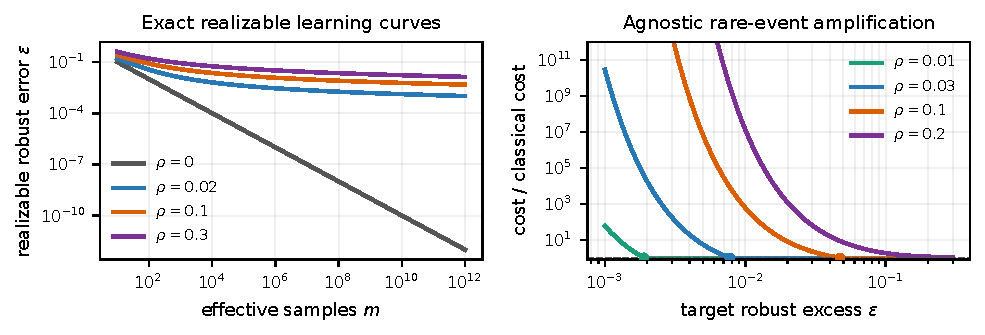
\includegraphics[width=0.98\linewidth]{kl_phase.pdf}
\caption{Exact robust accuracy scales from binary-KL inversion.  Left:
realizable target $\eps$ solving $B_\rho(\eps)=1/m$.  Any fixed positive radius eventually follows a logarithmic curve.  Right: agnostic effective minimax scale $\max\{\eps^{-2},B_\rho(\eps)^{-1}\}$ before the upper-bound logarithm, normalized by the classical $\eps^{-2}$ cost.  Dots mark the crossover $B_\rho(\eps)=\eps^2$.}
\label{fig:phase}
\end{figure}

\section{The inverse geometry behind the agnostic rate}
\label{sec:geometry}

Realizable learning follows immediately from the event reduction.  The agnostic result requires controlling $B_\rho$ at every possible optimal risk. The next theorem is the central new ingredient.

\begin{theorem}[Localized inverse spacing]
\label{thm:spacing}
There are universal $c>0$ and $\eps_0>0$ such that the following holds for $0<\eps\le\eps_0$ and every $\rho\ge0$.  Let $a=\min\{\eps^2,B_\rho(\eps)\}$.  For every $q\in[0,1-\eps]$, with $p=B_\rho(q)$,
\begin{equation}
 B_\rho(q+\eps)-B_\rho(q)
 \ge c\{a+\sqrt{ap}\}.
 \label{eq:spacing}
\end{equation}
\end{theorem}

We give the proof because it also explains the phase transition.  Joint convexity of binary KL implies that $Q_\rho$ is concave on its increasing part.  Hence $B_\rho$ is convex and
\begin{equation}
 B_\rho(q+\eps)-B_\rho(q)\ge B_\rho(\eps)=b.
 \label{eq:convex-spacing}
\end{equation}
For $p=B_\rho(q)$, implicit differentiation and the mean value theorem for the logit map give, for some $\xi\in(p,q)$,
\begin{equation}
 B_\rho'(q)=\frac{p(1-p)}{q-p}
 \log\frac{q(1-p)}{p(1-q)}
 =\frac{p(1-p)}{\xi(1-\xi)}\ge\frac pq.
 \label{eq:derivative}
\end{equation}

First suppose $b\ge\eps^2$.  Proposition~\ref{prop:inverse} implies $\rho\le\eps\log(1/\eps)$.  For $q\ge\eps$ it also gives \[ p\ge e^{-1}q\exp(-\rho/q)\ge c_0q^2, \] where the last inequality follows by maximizing $\log q+\eps\log(1/\eps)/q$ at an endpoint of $[\eps,1]$. Equation~\eqref{eq:derivative} now yields $B_\rho'(q)\ge\sqrt{c_0p}$.  Integration over an interval of length $\eps$, together with \eqref{eq:convex-spacing}, gives $\Delta B\gtrsim\eps^2+\eps\sqrt p$.  If $q\le\eps$, then $p\le b$ and \eqref{eq:convex-spacing} suffices.

Now suppose $b<\eps^2$.  Put $R=\rho/\eps$ and $r=q/\eps\ge1$. Proposition~\ref{prop:inverse} gives $R>\log(1/\eps)-1$ and
\begin{equation}
 \frac pb\ge e^{-1}r\exp\{R(1-1/r)\}\ge c_1r^2.
 \label{eq:ratio-pb}
\end{equation}
For completeness, subtracting $2\log r$ from the logarithm of the middle quantity reduces the claim to minimizing $R(1-1/r)-\log r$ on $[1,1/\eps]$.  Its minimum is at an endpoint and is bounded below universally.  Integrating \eqref{eq:derivative} correctly gives
\begin{equation}
 \Delta B\ge p\log(1+\eps/q)
 \ge\frac{p}{r+1}\ge\frac{p}{2r}gtrsim\sqrt{bp}.
 \label{eq:integrated-derivative}
\end{equation}
Combining this with \eqref{eq:convex-spacing} proves $\Delta B\gtrsim b+\sqrt{bp}$.  Again, $q\le\eps$ follows from $p\le b$. Appendix~\ref{app:geometry} supplies all endpoint and differentiability details.

\section{From scalar spacing to PAC bounds}
\label{sec:pac}

Let $p_\star=\inf_{h\in\cH}R_P(h)$ and let $\widehat h$ be ordinary ERM.  A relative VC inequality gives, with probability at least $1-\delta$,
\begin{equation}
 R_P(\widehat h)-p_\star
 \le C\left\{\sqrt{p_\star\Gamma/n}+\Gamma/n\right\},
 \quad
 \Gamma=d\log(2en/d)+\log(8/\delta).
 \label{eq:relative-vc}
\end{equation}
This standard form follows from relative-deviation symmetrization and peeling \citep{vapnik1971uniform,boucheron2005classification}.  A self-contained reduction from the uniform relative-deviation event is in Appendix~\ref{app:upper}.  This follows the scale-sensitive statistical strategy used at fixed Cressie--Read order by \citet{aignerhorev2026cressie}.  Theorem~\ref{thm:spacing} is the KL-specific ingredient that makes the strategy uniform at the endpoint.

Take $\Gamma/n\le c_2a$ for a sufficiently small universal $c_2$.  If $q_\star=Q_\rho(p_\star)>1-\eps$, criterion \eqref{eq:agnostic-criterion} is automatic.  Otherwise $p_\star=B_\rho(q_\star)$, and Theorem~\ref{thm:spacing} makes the right side of \eqref{eq:relative-vc} no larger than $B_\rho(q_\star+\eps)-B_\rho(q_\star)$.  Monotonicity then gives \[ Q_\rho(R_P(\widehat h))-Q_\rho(p_\star)\le\eps. \] Solving the mild implicit logarithm in $\Gamma$ proves the upper half of \eqref{eq:agn-rate}.

For the lower bound, the realizable subclass forces $\Omega((d+\log(1/\delta))/b)$.  When $b\ge\eps^2$, one has $\rho\le\eps\log(1/\eps)$.  At sufficiently small $\eps$, $Q_\rho'$ is bounded below by a universal constant on an interval around ordinary error $1/2$.  The standard noisy hypercube on a shattered set then converts each ordinary excess of order $\eps$ into robust excess of order $\eps$. Assouad testing gives $\Omega(d/\eps^2)$, and binary testing gives $\Omega(\log(1/\delta)/\eps^2)$.  Appendix~\ref{app:lower} gives the distributions, divergences, and constants.  This proves Theorem~\ref{thm:main}.

\section{Why the KL endpoint is singular}
\label{sec:endpoint}

The exponential is not obtained by inserting order one into constants proved for a fixed Cressie--Read order.  The following exact inequality is uniform at the endpoint.  For $s>0$, use
\begin{equation}
 D_{1+s}(q\|p)=
 \frac{q^{1+s}p^{-s}+(1-q)^{1+s}(1-p)^{-s}-1}{(1+s)s}
 \label{eq:cr}
\end{equation}
and let $B_{1+s,\rho}(q)$ be its lower inverse in $p$.

\begin{theorem}[Endpoint-uniform Cressie--Read bridge]
\label{thm:bridge}
For every $s>0$, $\rho\ge0$, and $0<q<1$, if $p=B_{1+s,\rho}(q)$, then
\begin{equation}
 \left[1+\frac{(1+s)s\rho}{q}\right]^{1/s}
 \le\frac qp\le
 \left[1+s+\frac{(1+s)s\rho}{q}\right]^{1/s}.
 \label{eq:bridge}
\end{equation}
For fixed $s$, this gives $B_{1+s,\rho}(q)\asymp_s q^{1+1/s}\rho^{-1/s}$ when $\rho/q\to\infty$.  As $s\downarrow0$, \eqref{eq:bridge} becomes
\begin{equation}
 e^{\rho/q}\le\frac{q}{B_\rho(q)}\le e^{1+\rho/q},
 \label{eq:bridge-limit}
\end{equation}
which is exactly Proposition~\ref{prop:inverse}.
\end{theorem}

To prove the display, put $r=q/p$.  The defining equation is \[ qr^s+(1-q)^{1+s}(1-q/r)^{-s}=1+(1+s)s\rho. \] The second term lies between $(1-q)^{1+s}$ and $1-q$, while $(1-q)^{1+s}\ge1-(1+s)q$.  Rearrangement gives \eqref{eq:bridge}.  Thus the fixed-order polynomial and the KL exponential are two limits of one finite inequality.  Together with the realizable reduction, it also yields an endpoint-uniform sample-complexity diagram.

\section{Discussion and limitations}

The result isolates a sharp statistical cost of support-preserving forward-KL robustness.  Ordinary ERM remains an empirical robust minimizer, yet fixed radius forces it to resolve exponentially rare nominal errors.  This explains why minimizer equivalence does not imply classical sample complexity.

Our scope is deliberately specific.  We study zero--one classification, distribution-free VC classes, and $D_{\mathrm{KL}}(Q\|P)$.  Reverse KL permits different support behavior.  General bounded losses need more than event inflation, and structural assumptions can improve distribution-free rates. The guarantees are information-theoretic, since ERM and the optimal realizable learner need not be computationally efficient for an arbitrary class.  The agnostic upper bound also retains the displayed logarithmic factor.  Removing it, or proving it unavoidable for this localized transform, is open.

\bibliography{references}
\bibliographystyle{iclr2027_conference}

\appendix

\section{Event reduction and inverse-map facts}
\label{app:event}

\subsection{Proof of Proposition~\ref{prop:event}}

Let $E$ have $P(E)=p$ and let $Q(E)=q$.  Applying the data-processing inequality for relative entropy to the indicator of $E$ gives $\KL(Q\|P)\ge\kl(q\|p)$.  Hence any feasible $q\ge p$ is at most $Q_\rho(p)$.

For $0<p<1$ and any $q\in[p,1]$, define \[ \frac{dQ}{dP}=\frac qp\mathbf 1_E+ \frac{1-q}{1-p}\mathbf 1_{E^c}. \] Then $Q(E)=q$ and $\KL(Q\|P)=\kl(q\|p)$, proving attainment.  If $p=0$, absolute continuity forces $q=0$.  If $p=1$, then $q=1$.  At $q=1$ the constraint is $\kl(1\|p)=\log(1/p)\le\rho$, which is equivalent to $p\ge e^{-\rho}$.  Strict monotonicity before this threshold follows from implicit differentiation, or directly from strict nesting of the feasible binary-KL intervals.

\subsection{Proof of Proposition~\ref{prop:inverse}}

For $p=B_\rho(q)$ in the interior,
\begin{equation}
 \rho=q\log\frac qp+(1-q)\log\frac{1-q}{1-p}.
 \label{eq:kl-inverse-equality}
\end{equation}
Because $p\le q$, the second term is nonpositive.  It is at least $-q$: write $x=(q-p)/(1-p)$ and use $\log(1-x)\ge-x/(1-x)$ to obtain \[ (1-q)\log\frac{1-q}{1-p} =(1-p)(1-x)\log(1-x)\ge-(q-p)\ge-q. \] Therefore \[ q\log(q/p)-q\le\rho\le q\log(q/p). \] Exponentiating proves \eqref{eq:inverse-bound}.  The endpoint cases follow by continuity.

\section{Complete proof of the spacing theorem}
\label{app:geometry}

The binary relative entropy is jointly convex.  Intersecting its $\rho$ sublevel set with the half-space $q\ge p$ gives the region between the diagonal and the upper graph of $Q_\rho$.  Convexity of that region implies concavity of $Q_\rho$ on $[0,e^{-\rho}]$.  Since this function is increasing, its inverse $B_\rho$ is convex.  In particular, for $q\ge0$ and $q+\eps\le1$,
\begin{equation}
 B_\rho(q+\eps)-B_\rho(q)
 \ge B_\rho(\eps)-B_\rho(0)=b.
 \label{eq:app-convex}
\end{equation}

For $0<p=B_\rho(q)<q<1$, differentiating \eqref{eq:kl-inverse-equality} gives \[ B_\rho'(q)=\frac{p(1-p)}{q-p} \left(\log\frac q{1-q}-\log\frac p{1-p}\right). \] The derivative of the logit is $1/[x(1-x)]$.  Thus the mean value theorem gives the equality in \eqref{eq:derivative}.  Since $p<\xi<q$, \[ \frac{B_\rho'(q)}{p/q} =\frac{q(1-p)}{\xi(1-\xi)}\ge1.
 \label{eq:app-derivative}
\] All integrations below can ignore endpoints and then pass to them by continuity.

Suppose first that $b\ge\eps^2$.  Equation \eqref{eq:kl-inverse-equality} and its nonpositive second term imply \[ \rho\le\eps\log(\eps/b)\le\eps\log(1/\eps). \] For $q\ge\eps$, Proposition~\ref{prop:inverse} gives \[ p\ge e^{-1}q\exp\left\{-\frac{\eps\log(1/\eps)}q\right\}. \] The function $f(q)=\log q+\eps\log(1/\eps)/q$ decreases and then increases, so its maximum on $[\eps,1]$ is at an endpoint.  The endpoint values are zero and $\eps\log(1/\eps)\le1/e$.  Hence $p\ge c_0q^2$ with $c_0=e^{-1-1/e}$.  By \eqref{eq:app-derivative}, \[ B_\rho'(q)\ge p/q\ge\sqrt{c_0p}. \] Monotonicity of $B_\rho$ then yields \[ B_\rho(q+\eps)-B_\rho(q) \ge\sqrt{c_0}\eps\sqrt{B_\rho(q)}. \] Together with \eqref{eq:app-convex} and $b\ge\eps^2$, this gives \eqref{eq:spacing} when $q\ge\eps$.  If $q\le\eps$, then $p\le b$ and $\eps\sqrt p\le b$, so \eqref{eq:app-convex} gives the result.

Now suppose $b<\eps^2$ and take $\eps_0\le e^{-2}$.  The lower half of \eqref{eq:inverse-bound} implies \[ R:=\rho/\eps>\log(1/\eps)-1. \] For $q=\eps r\ge\eps$, the two halves of \eqref{eq:inverse-bound} give \[ \frac pb\ge e^{-1}r\exp\{R(1-1/r)\}. \] To show this is at least $c_1r^2$, consider $g(r)=R(1-1/r)-\log r$.  Its derivative has the sign of $R-r$, so its minimum on $[1,1/\eps]$ occurs at an endpoint.  We have $g(1)=0$, while \[ g(1/\eps)\ge(\log(1/\eps)-1)(1-\eps)-\log(1/\eps) \ge-1-1/e. \] Thus one may take $c_1=e^{-2-1/e}$.

Using \eqref{eq:app-derivative} and monotonicity, we obtain the exact integral bound
\begin{align*}
 B_\rho(q+\eps)-B_\rho(q)
 &\ge\int_q^{q+\eps}\frac{B_\rho(u)}u\,du\\
 &\ge p\log(1+\eps/q)
 \ge\frac{p}{r+1}\ge\frac{p}{2r}
 \ge\frac{\sqrt{c_1}}2\sqrt{bp}.
\end{align*}
Combining with \eqref{eq:app-convex} gives $\Delta B\gtrsim b+\sqrt{bp}$.  When $q\le\eps$, $p\le b$, so the same conclusion follows directly from \eqref{eq:app-convex}.  This completes the proof.

\section{Upper bounds}
\label{app:upper}

We first record the only statistical input.  There is a universal $C$ such that ordinary ERM over a VC class satisfies, simultaneously for every $P$ and with probability at least $1-\delta$,
\begin{equation}
 R_P(\widehat h)-p_\star
 \le C\left\{\sqrt{p_\star\Gamma/n}+\Gamma/n\right\},
 \qquad
 \Gamma=d\log(2en/d)+\log(8/\delta).
 \label{eq:app-relative-vc}
\end{equation}
One route is the uniform relative-deviation event \[ |(P_n-P)(\ell_h-\ell_{h_\star})| \le C\left\{\sqrt{(P\ell_h+P\ell_{h_\star})\Gamma/n} +\Gamma/n\right\}. \] It follows by symmetrization, Sauer's lemma on the pooled sample, Bernstein's inequality, and peeling the true loss into dyadic intervals.  Since ERM has $P_n\ell_{\widehat h}\le P_n\ell_{h_\star}$, moving the resulting $\sqrt{(R_P(\widehat h)-p_\star)\Gamma/n}$ term to the left via $2\sqrt{uv}\le u/2+2v$ gives \eqref{eq:app-relative-vc}.  This is the usual relative VC inequality \citep{vapnik1971uniform,boucheron2005classification}. An infimum not attained is handled by a limiting sequence.

Let $a=\min\{\eps^2,b\}$.  If $n$ is such that $\Gamma/n\le c_0a$, then \eqref{eq:app-relative-vc} is at most \[ C\{\sqrt{c_0ap_\star}+c_0a\}. \] Choose $c_0$ so this is no greater than the right side of Theorem~\ref{thm:spacing}.  If $Q_\rho(p_\star)\le1-\eps$, spacing and monotonicity imply robust excess at most $\eps$.  If $Q_\rho(p_\star)>1-\eps$, every robust risk is at most one and the same conclusion is automatic.  Finally, $n\ge CA\{d\log(eA)+\log(1/\delta)\}$ makes the required inequality hold, after increasing $C$ to cover $n<d$.

In the realizable case, Proposition~\ref{prop:event} gives the exact equivalence \[ R_{\rho,P}(h)\le\eps\quad\Longleftrightarrow\quad R_P(h)\le b. \] Applying the optimal realizable VC upper bound at ordinary accuracy $b$ gives $O((d+\log(1/\delta))/b)$ samples.

\section{Lower bounds}
\label{app:lower}

We give the constructions to make clear that the two terms in \eqref{eq:agn-rate} arise from different experiments.

\subsection{Realizable rare-event lower bound}

For the worst-class lower bound, take $\cH$ to contain every labeling of $d$ points and a common label on one additional point.  This class has VC dimension $d$.  Assume $b\le1/16$, as follows from $\eps\le\eps_0$.  Give each of the first $d$ points mass $w=8b/d$ and the additional point the remaining mass.  Choose the labels on the first $d$ points uniformly from the $2^d$ realizable labelings.

For two target labelings differing only at coordinate $i$, their $n$-sample laws can be distinguished only if point $i$ appears.  Their total variation distance is therefore at most $1-(1-w)^n\le nw$.  Assouad's coordinate argument gives \[ \E H(\widehat\sigma,\sigma) \ge\frac d2(1-nw). \] If $n\le d/(64b)$, the right side is at least $7d/16$.  Since Hamming loss is at most $d$, this implies $\Pp\{H(\widehat\sigma,\sigma)\ge d/4\}\ge3/16$.  On that event the ordinary error is at least $2b>b$, so the robust risk exceeds $\eps$.

For confidence, use two realizable labelings differing on one point of mass $2b$.  Conditional on never observing that point, one of the two targets is misclassified there with probability at least one half.  Thus one target has failure probability at least $(1-2b)^n/2$.  For $b\le1/4$, this is at least $\delta$ whenever $n\le c\log(1/\delta)/b$.  The dimension and confidence bounds combine because their maximum is at least half their sum.  This proves the lower half of \eqref{eq:real-rate}, and also the $b^{-1}$ term in the agnostic lower bound.

\subsection{Agnostic noisy-label lower bound}

It remains to treat $b\ge\eps^2$.  Then $\rho\le\eps\log(1/\eps)$.  Choose $\eps_0$ so this is at most $1/32$. Pinsker's inequality implies $Q_\rho(p)-p\le\sqrt{\rho/2}$.  Hence, for $p\in[3/8,5/8]$, the point $q=Q_\rho(p)$ stays below $3/4$.  Inverting \eqref{eq:derivative} gives \[ Q_\rho'(p)=\frac{\xi(1-\xi)}{p(1-p)}\ge c_0
 \label{eq:Q-sensitivity}
\] for a universal $c_0>0$ and some $\xi\in(p,q)$.  Thus robust excess is at least $c_0$ times ordinary excess throughout this interval.

On $\mathcal X=\{1,\ldots,d\}$, let $\cH$ contain all binary labelings.  For $\sigma\in\{-1,1\}^d$, let $X$ be uniform and set \[ P_\sigma(Y=1\mid X=i)=\frac{1+\gamma\sigma_i}{2}. \] The optimal classifier has labeling $\sigma$, ordinary error $(1-\gamma)/2$, and a classifier with Hamming error $H$ has ordinary excess $\gamma H/d$.  Neighboring experiments have one-sample KL divergence at most \[ \frac1d\gamma\log\frac{1+\gamma}{1-\gamma} \le\frac{3\gamma^2}{d}, \] for $\gamma\le1/2$.  Pinsker's inequality and Assouad's argument yield $\E H\ge d/4$ whenever $n\le c d/\gamma^2$.  Adjusting constants gives $\Pp(H\ge d/8)\ge1/8$.  Take $\gamma=16\eps/c_0$.  For a smaller universal $\eps_0$, this is at most $1/4$, all risks lie in $[3/8,5/8]$, and Hamming error at least $d/8$ creates robust excess at least $2\eps$.  Therefore $n=\Omega(d/\eps^2)$ is necessary.

For the confidence term, use the two Bernoulli experiments with parameters $(1+\gamma)/2$ and $(1-\gamma)/2$.  Choosing the wrong constant classifier again creates robust excess at least $c_0\gamma$.  The Bretagnolle--Huber testing bound gives maximal error at least \[ \frac14\exp\{-3n\gamma^2\}. \] Taking $\gamma=2\eps/c_0$ proves $n=\Omega(\log(1/\delta)/\eps^2)$.  Combining this with the dimension bound and the realizable subclass completes the proof of Theorem~\ref{thm:main}.

\section{Proof of the Cressie--Read bridge}
\label{app:bridge}

Let $r=q/p\ge1$.  Multiplying the equality $D_{1+s}(q\|p)=\rho$ by $(1+s)s$ gives
\begin{equation}
 qr^s+(1-q)^{1+s}(1-q/r)^{-s}=1+(1+s)s\rho.
 \label{eq:app-cr-root}
\end{equation}
Since $q/r=p\le q$, \[ (1-q)^{1+s}le (1-q)^{1+s}(1-q/r)^{-s}\le1-q. \] The upper inequality follows because $[(1-q)/(1-p)]^s\le1$.  Convexity also gives $(1-q)^{1+s}\ge1-(1+s)q$.  Substituting the upper bound on the complement term into \eqref{eq:app-cr-root} yields \[ r^s\ge1+(1+s)s\rho/q. \] Substituting its lower bound and then the tangent inequality yields \[ r^s\le1+s+(1+s)s\rho/q. \] Taking $s$th roots proves \eqref{eq:bridge}.  The fixed-$s$ asymptotic is immediate.  Pointwise convergence of $D_{1+s}$ to forward KL, together with uniqueness and monotonicity of the lower root, gives $B_{1+s,\rho}(q)\to B_\rho(q)$.  Finally, $(1+sx)^{1/s}\to e^x$ and $(1+s+s(1+s)\rho/q)^{1/s}\to e^{1+\rho/q}$, which proves \eqref{eq:bridge-limit}.

\section{Exact numerical diagnostics}
\label{app:numerics}

Figure~\ref{fig:phase} and all diagnostics use bisection on the scalar equation $\kl(q\|p)=\rho$.  No Monte Carlo samples or fitted parameters enter the plots.  As a guard against algebraic errors, we tested 80 pairs $(\eps,\rho)$ over 240 values of $q$ each.  The smallest normalized spacing was $0.9844$, and the largest ratio of the gridded localized-complexity expression to $\max\{\eps^{-2},B_\rho(\eps)^{-1}\}$ was $1.0000$.  We also tested 500 random Cressie--Read roots.  Every root lay inside \eqref{eq:bridge}, with the closest normalized distances to the lower and upper boundaries equal to $1.00009$ and $0.999999$.  These computations are reproducibility checks, not inputs to any proof.

\end{document}
